We propose to study photoproduction of lepton pairs,
$\gamma p \to l^+l^-p^\prime$, in a wide range of kinematics using the
SoLID detector in Hall A and a 11 GeV longitudinally polarized electron beam
impinging on a hydrogen target.
The analysis will use the fully exclusive electroproduction reaction:
\begin{equation}
ep \to e^+e^-p^\prime(e^\prime) \
\label{eq:exfs}  
\end{equation}
where the initial electron (e$^\prime$) scatters at a small angle
($\sim 0^\circ$), and escapes detection in SoLID. In Eq.~(\ref{eq:exfs}),
$e^+e^-$ is the produced lepton pair, and $p^\prime$ is the recoil proton.
The main goal of the measurement is to extract cosine and sine moments of the
weighted cross section, and the five-fold differential cross section:
\begin{equation}
\frac{d^5\sigma}{dQ^{\prime 2}dtd\eta d(\cos{\theta_{CM}})d(\varphi_{CM})} \
\label{eq:diffxs}
\end{equation}
for several bins of $\eta$, $t$, $Q^{\prime 2}$, and the lepton polar and
azimuthal angles $\theta_{CM}$ and $\varphi_{CM}$ in the 
(e$^+$e$^-$) Center-of-Mass system, respectively.
The longitudinal and transverse momentum components of the scattered
beam electron will be deduced from missing momentum analysis. 

This final state contains two leptons and a proton, which can provide a
coincidence trigger. To suppress background from two-pion photoproductio, the
trigger has to contain the two leptons, at least one of which should also be
within the acceptance of the Cherenkov. The data can be collected in parallel
with any SoLID experiment with similar trigger requirement, {\it e.g.}, the
SoLID $J/\psi$ electroproduction experiment E12-12-006~\cite{E12-12-006}.
If there is a need to reduce the rate further, an additional condition of
a third track (the proton) can be added.
The base equipment and DAQ of SoLID are suitable for conducting these
measurements, but an additional TOF detector covering large polar angles
(see Sect.~\ref{sec:detector}) would be needed. The exclusivity of the
reaction is ensured by detecting all final-state particles, $e^+e^-p$ and
cutting on the missing-particle kinematics (transverse momentum and missing
mass), in a similar manner as in the TCS analysis of the CLAS 6 GeV
data~\cite{Rafael:2010}.

\subsection{The SoLID detector}
\label{sec:detector}

\begin{figure}[t]
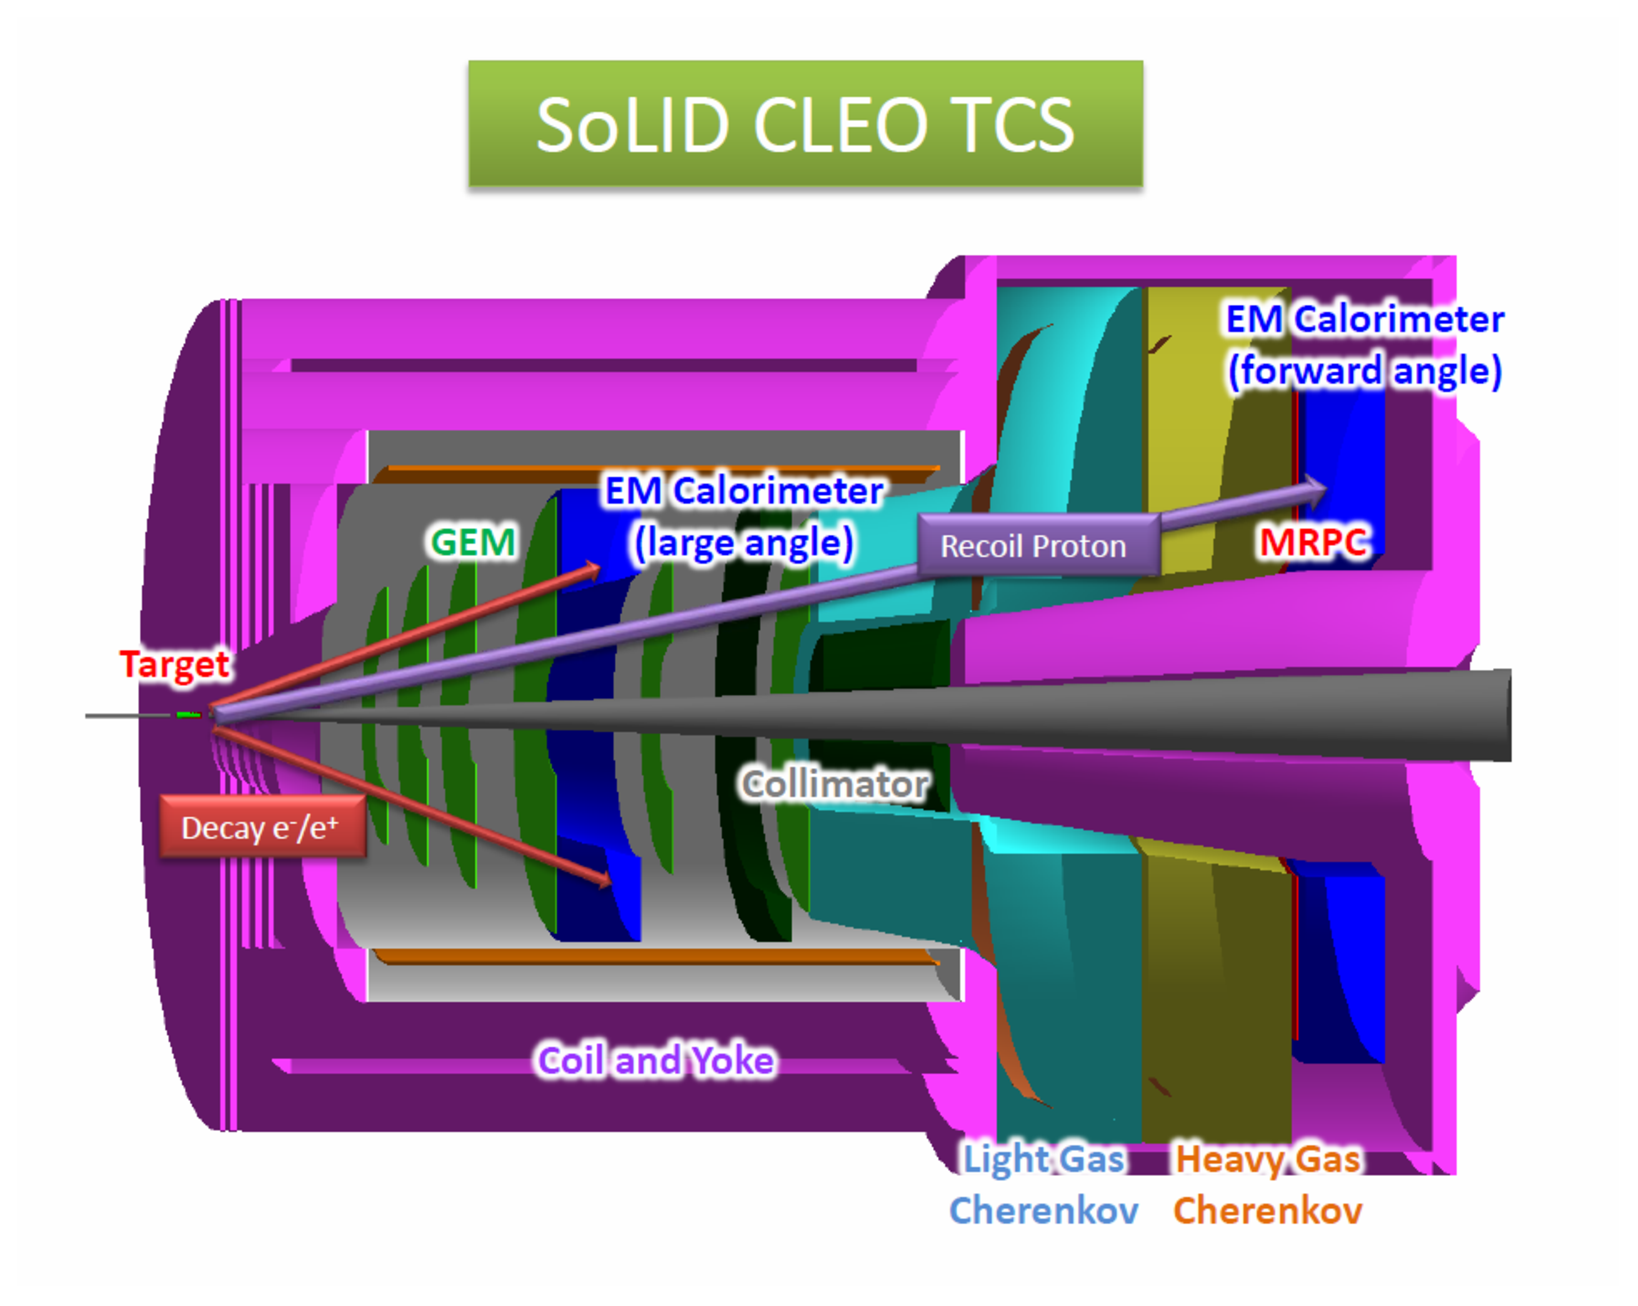
\includegraphics[width=125mm]{SoLID_setup_20130225_TCS_arrow.eps}
\caption{\small{The SoLID detector in Hall A.}}
\label{fig:solid}
\end{figure}

\begin{table}[t]
 \centering
 \begin{tabular}{|l|c|}
\hline
Parameters                                    & SoLID detector \\ 
\hline
polar angular range ($\theta$)       & $8^\circ$ to $17^\circ$ and $18^\circ$ to $28^\circ$  \\ 
azimuthal angular range ($\phi$)   & full  \\ 
resolution: &     \\ 
~~~polar angle ($\delta\theta$)     & $<0.6$ mr  \\ 
~~~azimuthal angle ($\delta\phi$) &$<5$ mr \\ 
~~~momentum ($\delta$p/p)         &$<2\%$ \\ 
\hline
PID: &\\
~~~~~~~e/$\pi$ by EC & full momentum range \\
~~~~~~~e/$\pi$ by CC & $<5$ GeV/c at $8^\circ < \theta <17^\circ$ \\
~~~~~~~p/K by TOF    & $<4.5$ GeV/c at $8^\circ < \theta <17^\circ$ and $<2.5$ GeV/c at $18^\circ < \theta <28^\circ$ \\ 
\hline
\end{tabular}
\caption{SoLID design characteristics.}
\label{table:SoLID}
\end{table}

SoLID, shown in Fig. \ref{fig:solid} will be an all-new detector in Hall A
during the 12 GeV era. It is designed to use a solenoid field to sweep away
low-energy charged background particles, and can thus carry out experiments
using high-energy electron beams incident on unpolarized or polarized targets
at luminosities up to $L=10^{37}$ cm$^{-2}$ sec$^{-1}$ in an open geometry.
It has two groups of the detectors. The forward-angle detectors cover polar
angle from $8^\circ$ to $17^\circ$ and consist of several planes of Gas
Electron Multipliers (GEM) for tracking, a light-gas Cherenkov (LGCC) for
e/$\pi$ separation, a heavy gas Cherenkov (HGCC) for $\pi$/K separation,
a Multi-gap Resistive Plate Chamber (MRPC) for time-of-flight, and an
Electromagnetic Calorimeter (FAEC).
The large-angle detectors covers polar angle from $18^\circ$ to $28^\circ$
and consist of several planes of GEM for tracking, an MRPC for time of flight
(new for TCS), and an Electromagnetic Calorimeter (LAEC). The design
characteristics of SoLID are presented in Table \ref{table:SoLID}. Particles
in SoLID will be detected and identified by measuring their momenta,
time-of-flight, number of photons produced in the threshold Cherenkov
counters, and energy losses in the calorimeters and MRPC.

The SoLID solenoid will reuse the CLEO-II magnet. Its superconducting coil and
cryo will remain the unchanged. It has a large inner space with a clear bore
diameter of 2.9 m and a coil of 3.1 m diameter. The coil length is 3.5 m, with
a 3.8 m long cryostat. The coil is made of  $5 \times 16$ mm$^2$
aluminum-stabilized superconductor, and runs at 3300 A.
Part of the CLEO-II iron flux return will be modified and reused, and two new
iron endcaps will be added at the front and back of the solenoid. The axial
central field of the solenoidal magnet can reach about 1.4 T.

Six layers of GEM detectors will be used for tracking, providing information
on the momentum, angle, and interaction vertex of the detected particles. They
will be placed uniformly inside the solenoid magnet. For the forward angle
detectors, five layers
%(except for the first layer)
of GEM detectors will be used. In principle, three points are needed to
reconstruct the kinematic variables. The fourth and fifth points will bring
enough redundancy to compensate for the inefficiency of the GEM tracking
detector. For the large-angle detectors, four layers of GEMs detector will be
used. In this case, four layers are enough since the background level at
large angles is expected to be smaller. SoLID GEMs will provide full azimuthal
angular coverage by using trapezoidal-shaped sectors. The area of a single
sector can be as large as 100 cm $\times$ 40 cm. Recent advancements in
technology, like single-mask GEM etching and GEM splicing, makes it possible
to fabricate GEM foils up to 100 cm $\times$ 200 cm. The GEM readout is by
2D strips and APV-25 based chips from the funded Scalable Readout System (SRS)
project by the CERN RD-51 collaboration.

The Cherenkov detectors (CC) at forward angles have two parts. The light-gas
one uses a standard $CO_2$ gas radiator and can provide e/$\pi$ separation up
to momenta of 5 GeV/c with pion rejection in order of $10^3$. The heavy-gas
one uses $C_4F_8O$ gas at 1.5 atm and gives a momentum threshold of 2.2 GeV/c
and 7.5 GeV/c for pions and kaons, respectively. In both cases, the Cherenkov
light is directed by the mirror systems onto Multi-Anode PMTs (MAPMTs) for
readout. The MAPMTs have been tested to work with longitudinal magnetic fields
up to 400 G.

There is one electromagnetic calorimeter at forward angles and one at large
angles. They are made with identical Shashlyk-type modules. Each module is
made of a pre-shower and a shower part. The pre-shower detector is simply a
2 radiation-length lead layer and a 2 cm thick scintillator with embedded
wave-length-shifting (WLS) fibers for readout. The shower detector is of
Shashlyk type, consisting of about 200 layers of 0.5 mm lead and 1.5 mm
scintillator, and many WLS fibers penetrating all layers with a density about
$1/$cm$^2$ for readout at the back of a module. This type of design can reach
a pion rejection factor of more than 100, with good electron efficiency. Its
radiation hardness is in the order of 500 krad, which satisfies the
high-luminosity condition in SoLID.

MRPC-based time-of-flight systems have recently been used in the RHIC STAR and
LHC ALICE experiments, providing a typical time resolution close to 80 ps.
With readout strips, it can work inside a magnetic field. Using low-resistive
glass, it can gain even an higher rate capability. SoLID experiments have a
forward-angle MRPC as part of the planned baseline equipment. This experiment
needs a large-angle MRPC between the last GEM plane and the large-angle EC to
identify recoil protons at large angles. Its 5 m$^2$ area is about half that
of the forward-angle MRPC, and the cost is also estimated to be about half,
or about \$500k.

\subsection{Detection of exclusive $e^+e^-p$ events}
\label{sec:tcs_selection}

The simulations of the SoLID detector for the proposed measurements used an 11
GeV electron beam and a 15 cm long liquid hydrogen target. Exclusive
$e^+e^-p$ events, with invariant masses of the lepton pairs in the
resonance-free region between 2 and 3 GeV, were generated over a wide range of
kinematics by using the standalone event generator genTCS~\cite{genTCS}. Both
quasi-real photons from electron scattering, according to the equivalent
photon approximation (EPA)~\cite{Kessler:1994}, and real photons from
Bremsstrahlung~\cite{PDG:2012} on the target were included. (The former is
dominant in the configuration of this experiment.) Each event was weighted by
the Bethe-Heitler (BH) cross section from Ref.~\cite{Berger:2001xd}. The
response of the detector was simulated using the SoLID simulation package
SoLID GEMC~\cite{SoLID_GEMC}.

SoLID does electron and positron identification by combining CC and EC
information at the forward angles, and uses only the EC at the large angles.
The CC can offline provide a single-pion rejection factor of about 1000, and
the EC can do a factor of 100. To suppress the large (0.1 mb) background from
two-pion photoproduction, we require that at least one lepton is detected
within the CC acceptance at forward angles and has momentum less than 5 GeV,
which is the SoLID light-gas Cherenkov e/$\pi$ separation threshold. This will
ensure a pion-pair rejection factor of at least $10^7$, which is sufficient to
cleanly separate out the lepton-pair events from the pion background.
Fig.~\ref{fig:eid} shows the momentum- and angular distribution of two leptons
detected in SoLID. The events with both leptons going into the large-angle
detectors are discarded, and a momentum cut is applied for the leptons going
to the forward angles.

\begin{figure}[t]
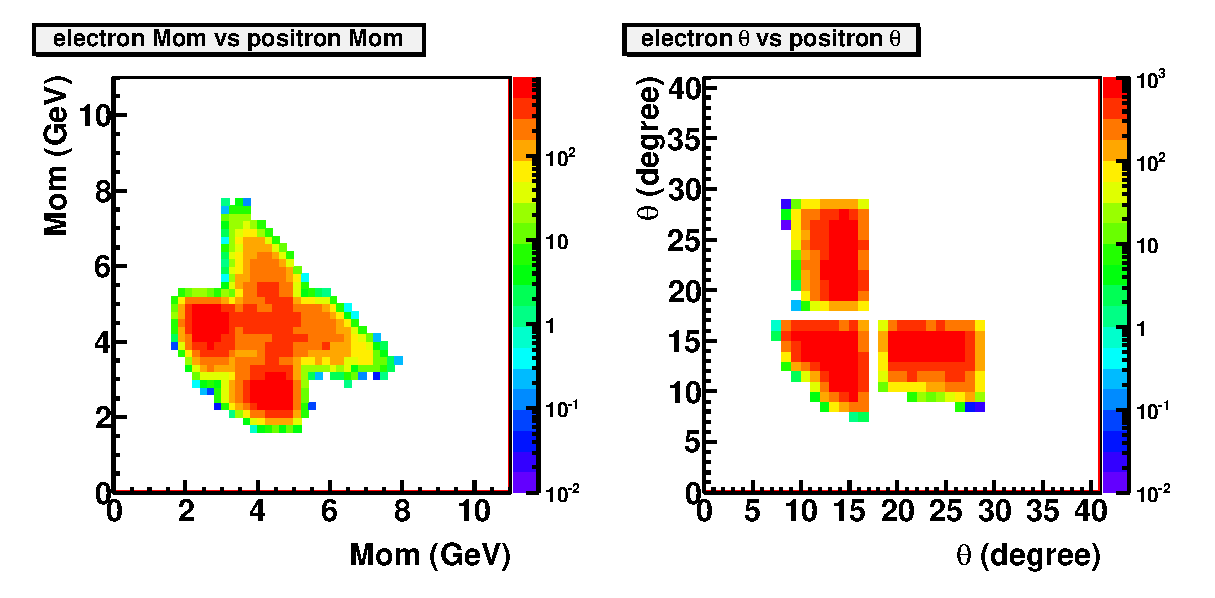
\includegraphics[width=125mm]{ep_final.eps}
\caption{\small{Decay lepton pair detected by CC and EC
{\it Left panel:} Electron momentum versus positron momentum.
{\it Right panel:} Electron polar angle versus positron polar angle.}}
\label{fig:eid}
\end{figure}

Protons are mainly identified in SoLID by time-of-flight using the MRPC. With
a time resolution at about 80 ps and flight path of about 750 cm for forward
angles and 250 cm for large angles, protons with momenta up to 4.6 GeV and 2.5
GeV, respectively, can be identified by the MRPC, as shown in
Fig.~\ref{fig:hid}. This allows access to a wide range in t.

\begin{figure}[t]
\begin{center}
\mbox{\subfigure{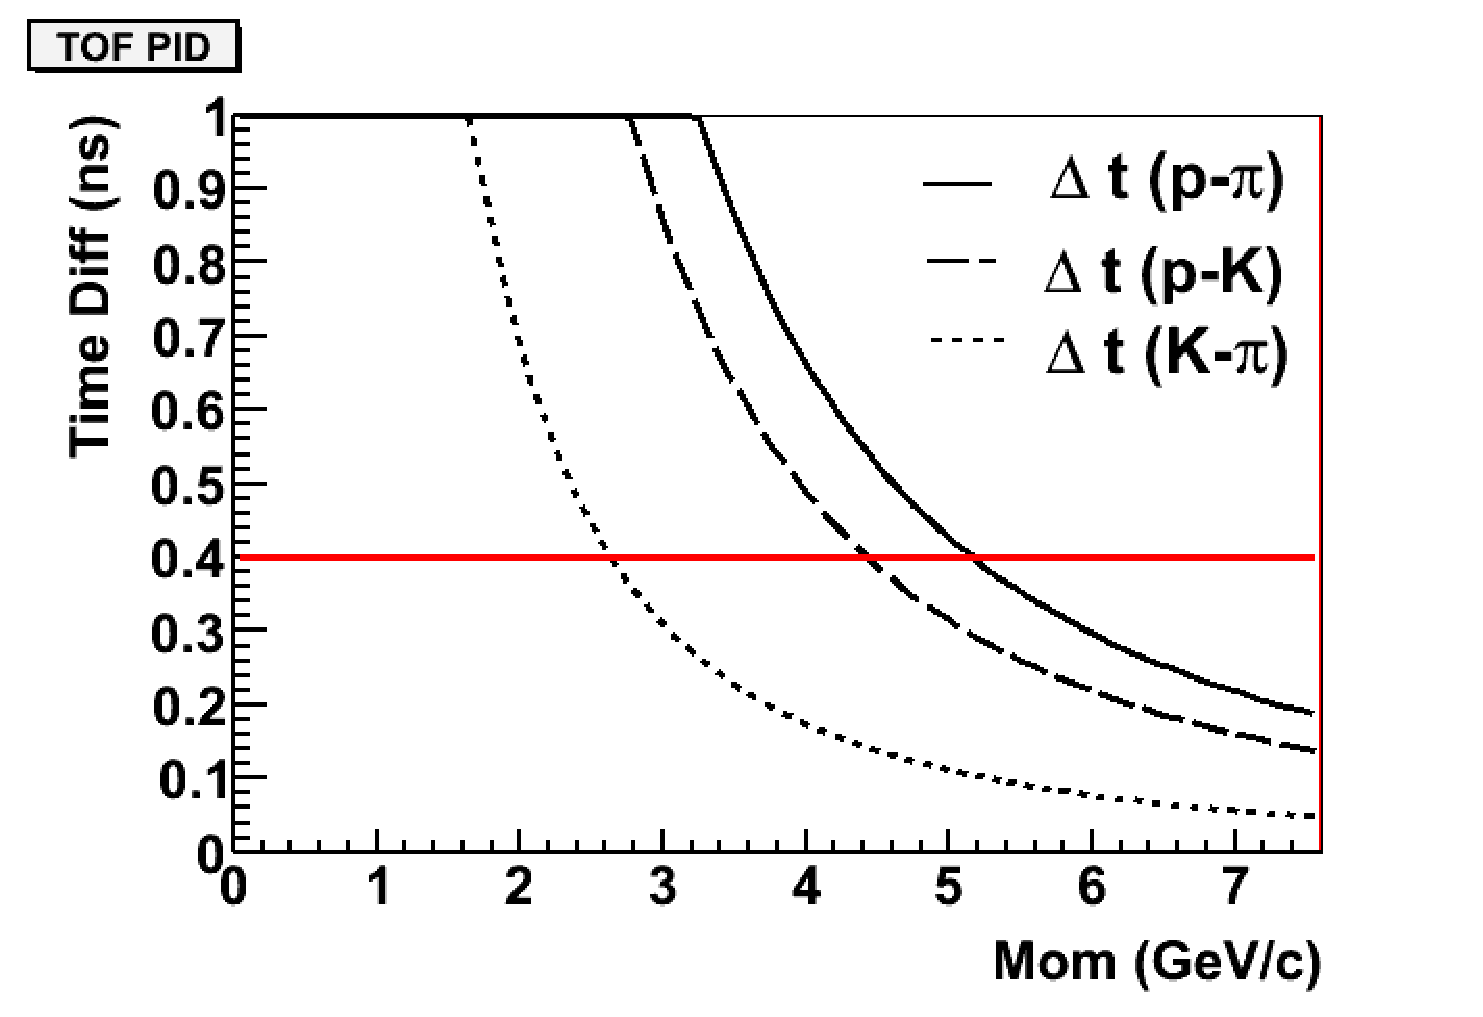
\includegraphics[width=64mm]{tofpid_SIDIS_FA.eps}} \quad
\subfigure{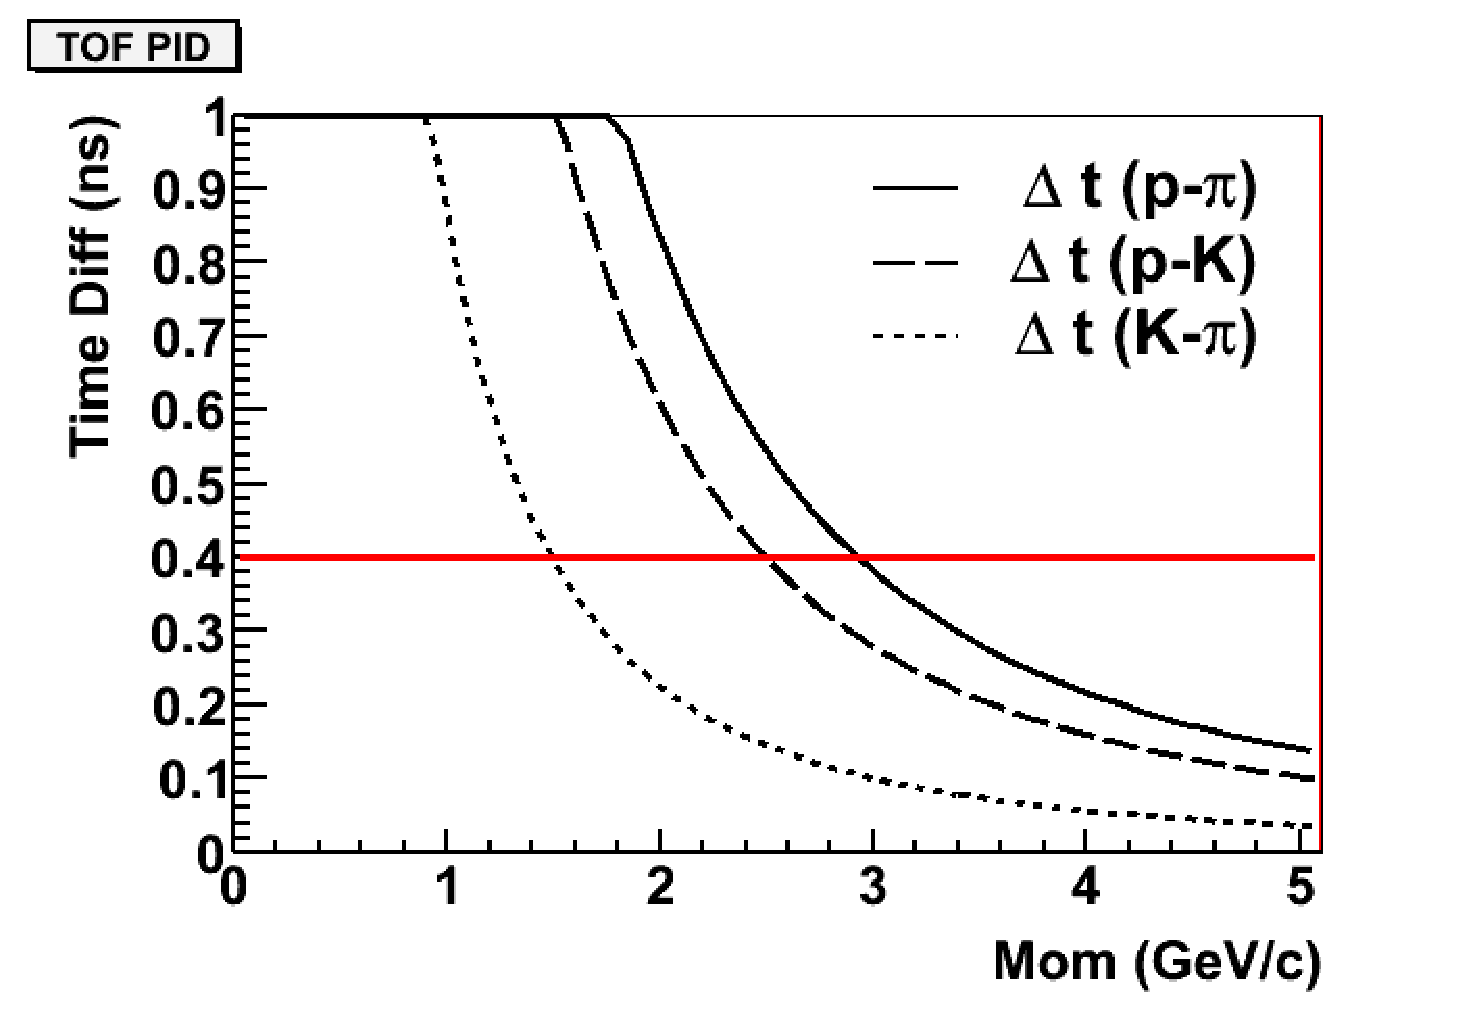
\includegraphics[width=65mm]{tofpid_TCS_LA.eps} } }
\end{center}
\caption{\small{Proton PID by TOF in the MRPC. The graphs show the time
difference vs. momentum for kaons and pions, protons and kaons, and protons
and pions for the forward angles ({\it left panel:}) and the large angles
({\it right panel:}). The horizontal lines shows where a $5\sigma$ separation
with 80 ps time resolution is. The intersecting point of the horizontal line
with the protons and kaons time difference line determines the max momentum
of proton identification.}}
\label{fig:hid}
\end{figure}

Fig.~\ref{fig:theta_mom} shows the momentum and polar angle distribution
of $e^+$, $e^-$, p, and the missing electron from the simulated BH events
with invariant mass of lepton pairs 2 GeV $< Q^\prime < 3$ GeV. The decay
lepton has momentum from 2 to 8 GeV. The recoil protons mostly have momenta
below 1.5 GeV/c. The energy of the missing electron reconstructed from the
detected lepton pairs and protons are ranging from 6 to 11 GeV.

\begin{figure}[t]
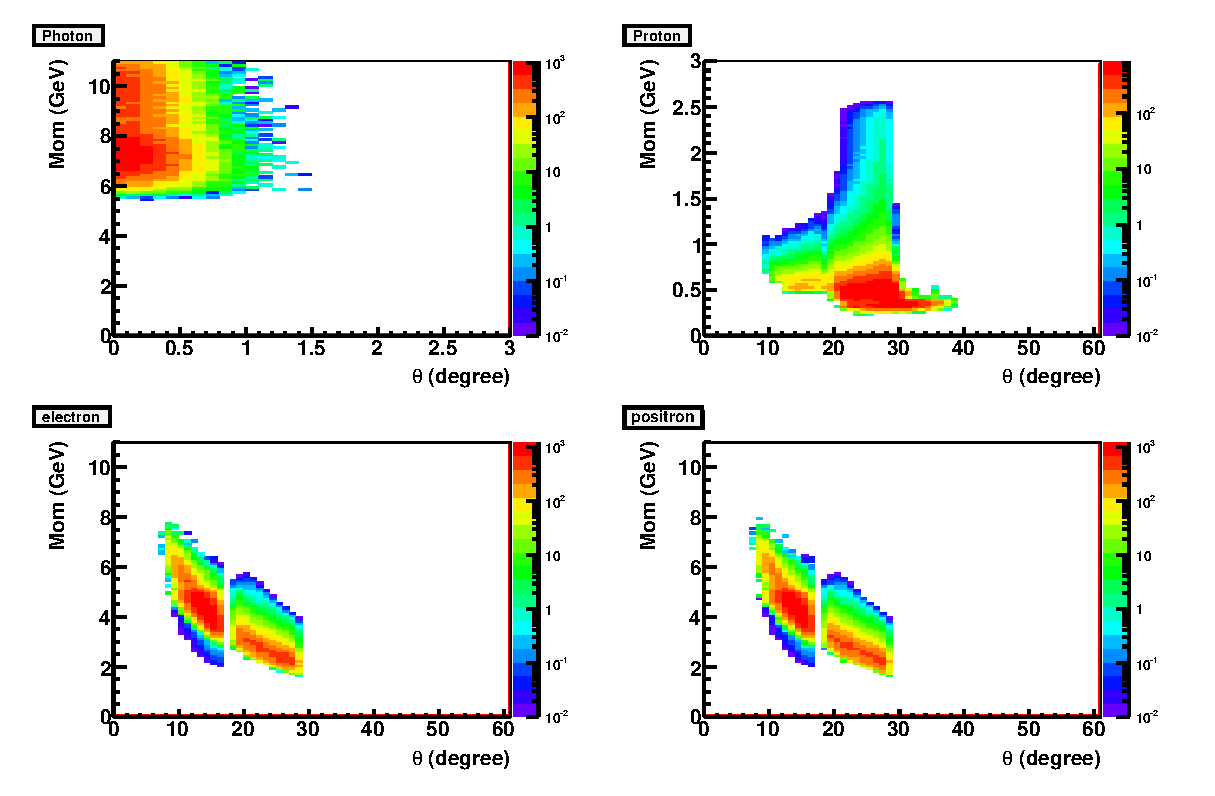
\includegraphics[width=125mm]{theta_mom_final.eps}
\caption{\small{Momentum and polar angle distribution of the missing
beam electron, recoil proton, decay electron, and decay positrion}}
\label{fig:theta_mom}
\end{figure}

To ensure exclusivity of the reaction, cuts need to be applied on the missing
particle kinematics. The missing particle can be a very forward scattered
electron in quasi-real electroproduction, or an electron that radiated a real
photon in photoproduction. In the latter case, the $Q^2$ is identically zero,
and in the former it is kept close to zero through cuts on the missing mass
missing transverse momentum.
In the simulation, the detected $e^+e^-p$ momenta and angles were smeared by
the SoLID detector resolution, thus creating a realistic distribution of
kinematic variables for the missing particle. Instead of applying cuts on the
transverse momentum, a corresponding cut of $Q^2 < 0.05$ GeV$^2$ was applied.
Fig.~\ref{fig:Miss_2D} shows the kinematic variables of the missing particle
before and after the cut. As can be seen, the SoLID momentum- and angular
resolution is sufficient for cleanly identifying exclusive events with
quasi-real photons.

\begin{figure}[t]
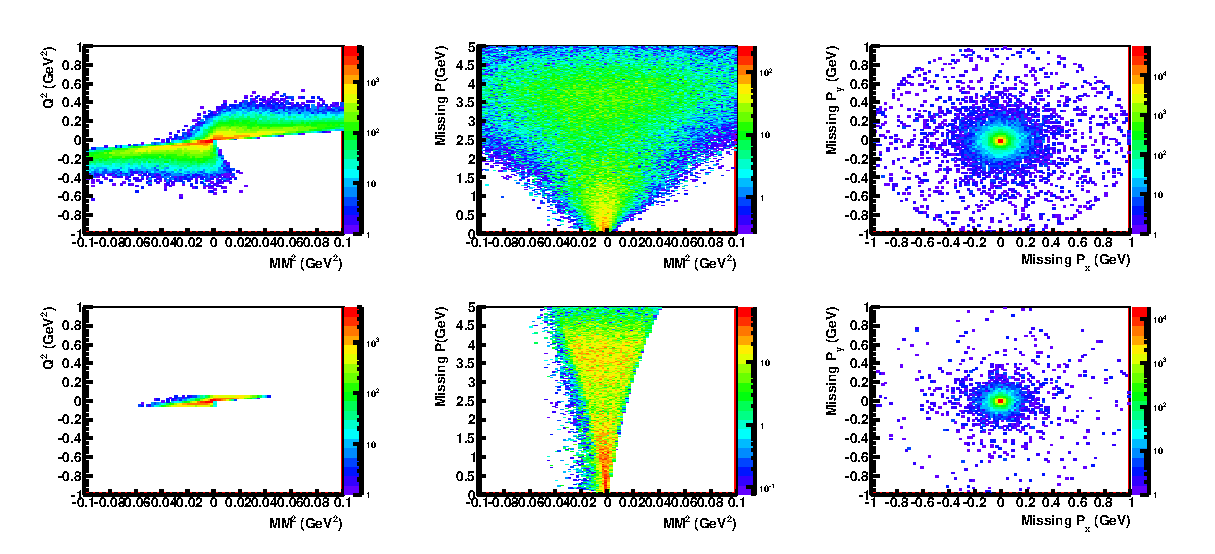
\includegraphics[width=125mm]{Miss_2D.eps}
\caption{\small{Missing-particle kinematics before and after the cut
$Q^2 < 0.05$ GeV$^2$
{\it Left panels:} $Q^2$ versus missing mass squared $MM^2$.
{\it Middle panels:} Missing momentum versus missing mass squared $MM^2$.
{\it Right panels:} Missing momentum P$_x$ versus missing momentum P$_y$.
{\it Top row:} before the $Q^2$ cut
{\it Bottom row:} after the $Q^2$ cut.}}
\label{fig:Miss_2D}
\end{figure}
